%META {"title":"Hình bình hành","note":"AB // DC và AD // BC (hai cặp cạnh đối của hình bình hành). HS trả lời miệng: dùng góc so le trong với đường chéo BD, hoặc đồng vị — vì sao hai cạnh đối song song."}
\documentclass[border=5pt]{standalone}
\usepackage{tkz-euclide}
% Màu dùng chung cho toàn bộ hình vẽ (ảnh stack với nền tối của web)
\definecolor{tminc}{RGB}{226,232,240}   % chữ + nét chính
\definecolor{tmblue}{RGB}{0,210,255}    % nhấn neon xanh
\definecolor{tmpink}{RGB}{255,0,200}    % nhấn neon hồng
\definecolor{tmgreen}{RGB}{0,255,136}   % nhấn neon xanh lá
\color{tminc}

\begin{document}
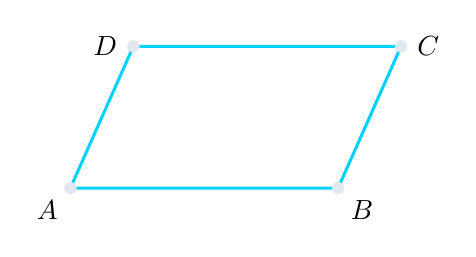
\begin{tikzpicture}[line width=1.1pt]
  \coordinate (A) at (0,0);
  \coordinate (B) at (3.4,0);
  \coordinate (C) at (4.2,1.8);
  \coordinate (D) at (0.8,1.8);
  \tkzDrawPolygon[tmblue,line width=1.1pt](A,B,C,D)
  \tkzDrawPoints[size=3.5,color=tminc,fill=tminc](A,B,C,D)
  \tkzLabelPoint[below left=1pt](A){$A$}
  \tkzLabelPoint[below right=1pt](B){$B$}
  \tkzLabelPoint[right=2pt](C){$C$}
  \tkzLabelPoint[left=2pt](D){$D$}
\end{tikzpicture}
\end{document}
